\chapter{Produkteinsatz}

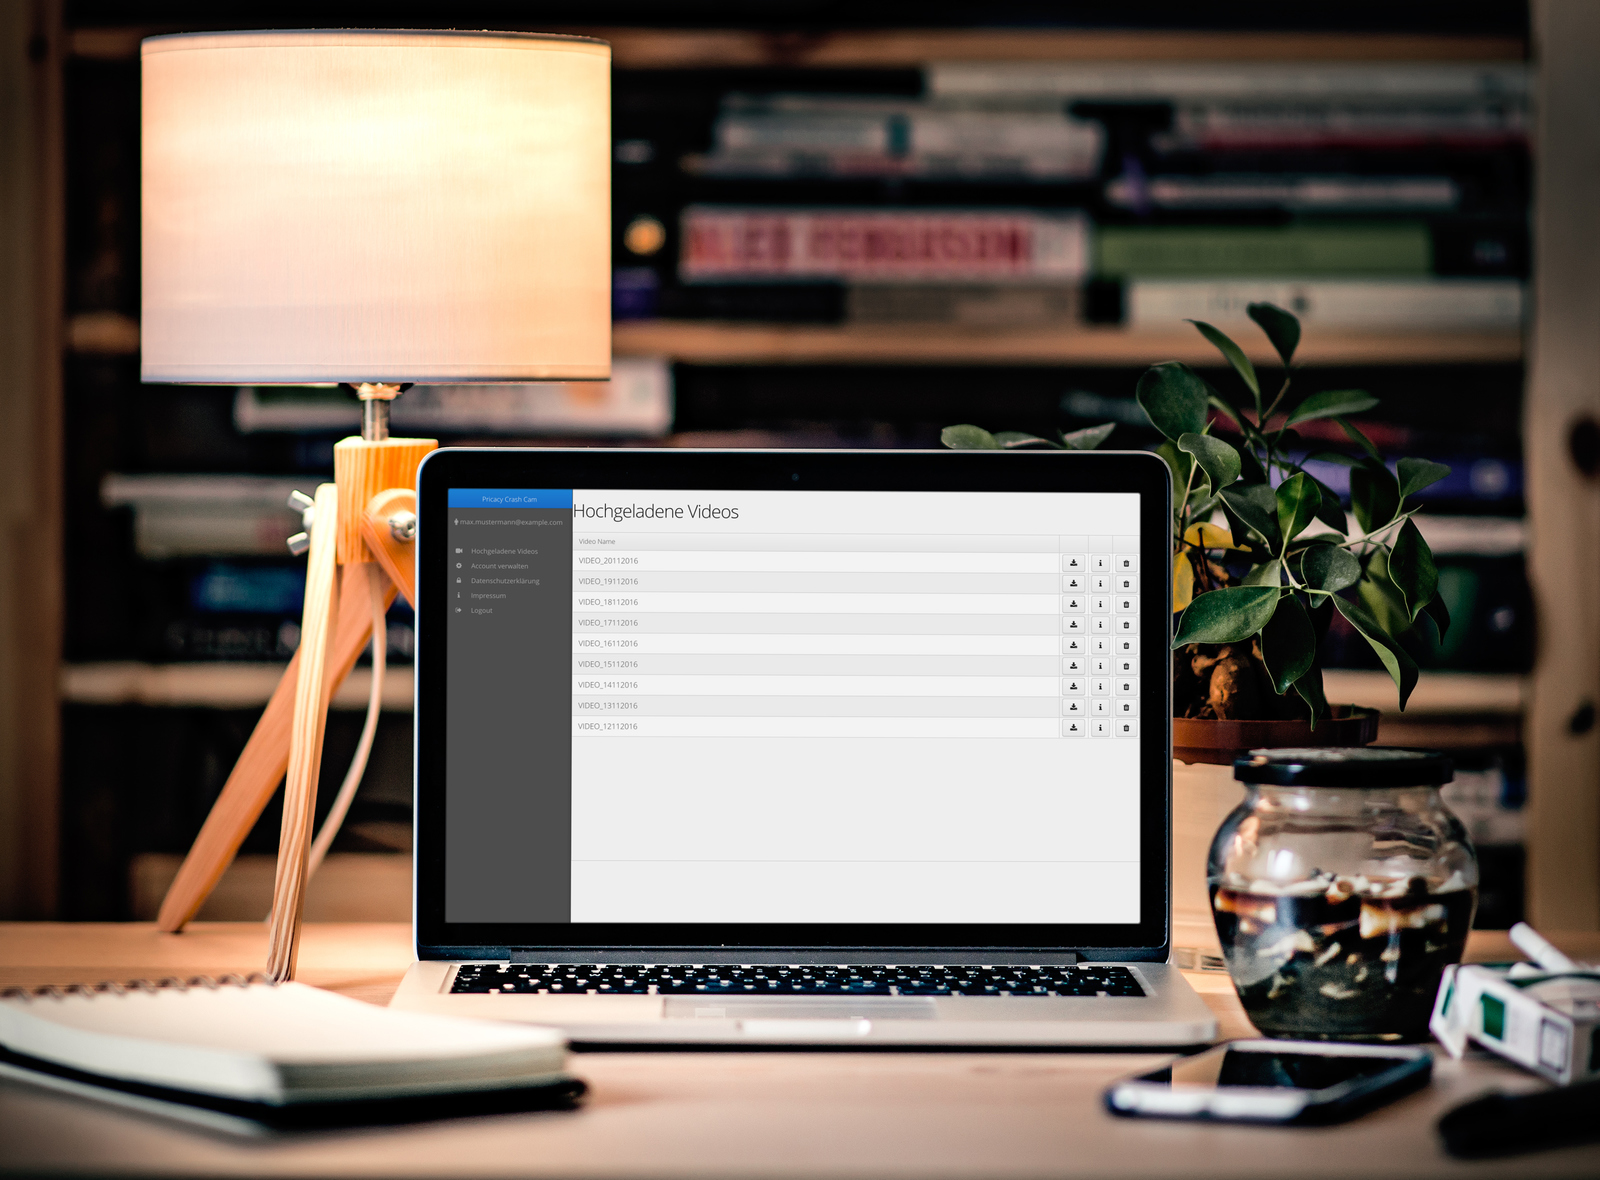
\includegraphics[width=\textwidth]{subtopicsFuncspec/Res/Mockups/Webinterface_desktop.jpg}

\section{Zielgruppe}
Die Privacy Dash Cam verfolgt zwei grundlegende Ziele: Eine Dash Cam für das \gls{Smartphone} anzubieten und ihren Einsatz mit dem deutschen Datenschutzrecht in Einklang zu bringen. Daraus lässt sich eine eindeutige Zielgruppe ableiten, die sich aus in Deutschland und Österreich ansässigen Auto-, LKW- und Motorrad-Fahrern zusammensetzt. Dabei haben sowohl Viel- als auch Gelegenheitsfahrer Bedarf an der Privacy Dash Cam. Darüber hinaus müssen Nutzer ein \gls{Smartphone} besitzen, welches den Geräteanforderungen der \gls{App} gerecht wird. Weiterhin werden Kenntnisse über die Benutzung des \glslink{Smartphone}{Smartphones}, Verständins der deutschen Sprache und ein Internetzugang für die Verwendung des Produktes vorausgesetzt.

\section{Einsatz}
Nachdem die \gls{App} auf einem kompatiblen \gls{Smartphone} installiert und ein Nutzeraccount erstellt wurde, findet sie ihren Einsatz im Straßenverkehr. Der Nutzer platziert dazu sein \gls{Smartphone} mithilfe einer speziellen Halterung an der Frontscheibe seines Kraftfahrzeugs und ermöglicht so der Kamera ein deutliches Bild auf die Straße vor ihr. Darüber hinaus wird das \gls{Smartphone} nach dem Aufzeichnen von relevantem Videomaterial verwendet, um besagtes Material dem Webservice zum \glslink{anonymisieren}{Anonymisieren} zu senden.\newline
Das Web-Interface stellt die zweite Instanz dar, mit der der Nutzer direkt interagieren kann. Mit Hilfe dieser kann der Nutzer seinen Account verwalten und das vom \gls{Web-Dienst} \glslink{anonymisieren}{anonymisierte} Videomaterial herunterladen.

